\section{Auswertung}
\label{sec:Auswertung}


\subsection{Blockschaltbild}

\begin{figure}[H]
    \centering
    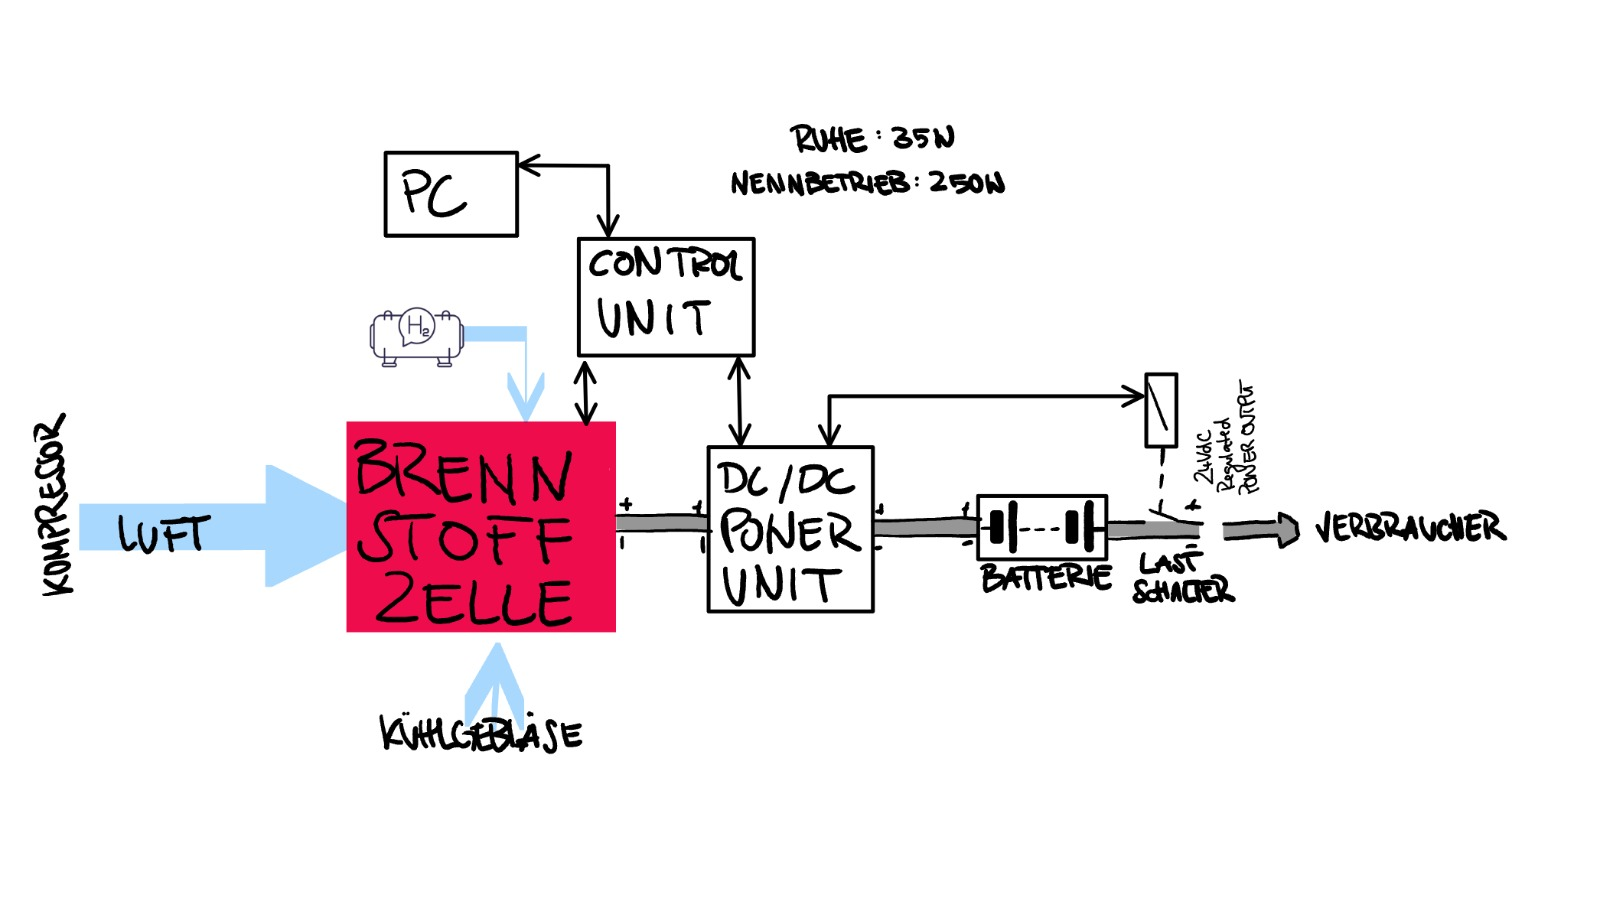
\includegraphics[width=\textwidth]{Abbildungen/Brennstoffzelle_Blockschaltbild.jpeg}
    \caption{Blockschaltbild}
    \label{fig:230628_Blockschaltbild}
\end{figure}


\subsection{Grafische Darstellung Messdaten}

\begin{figure}[H]
    \centering
    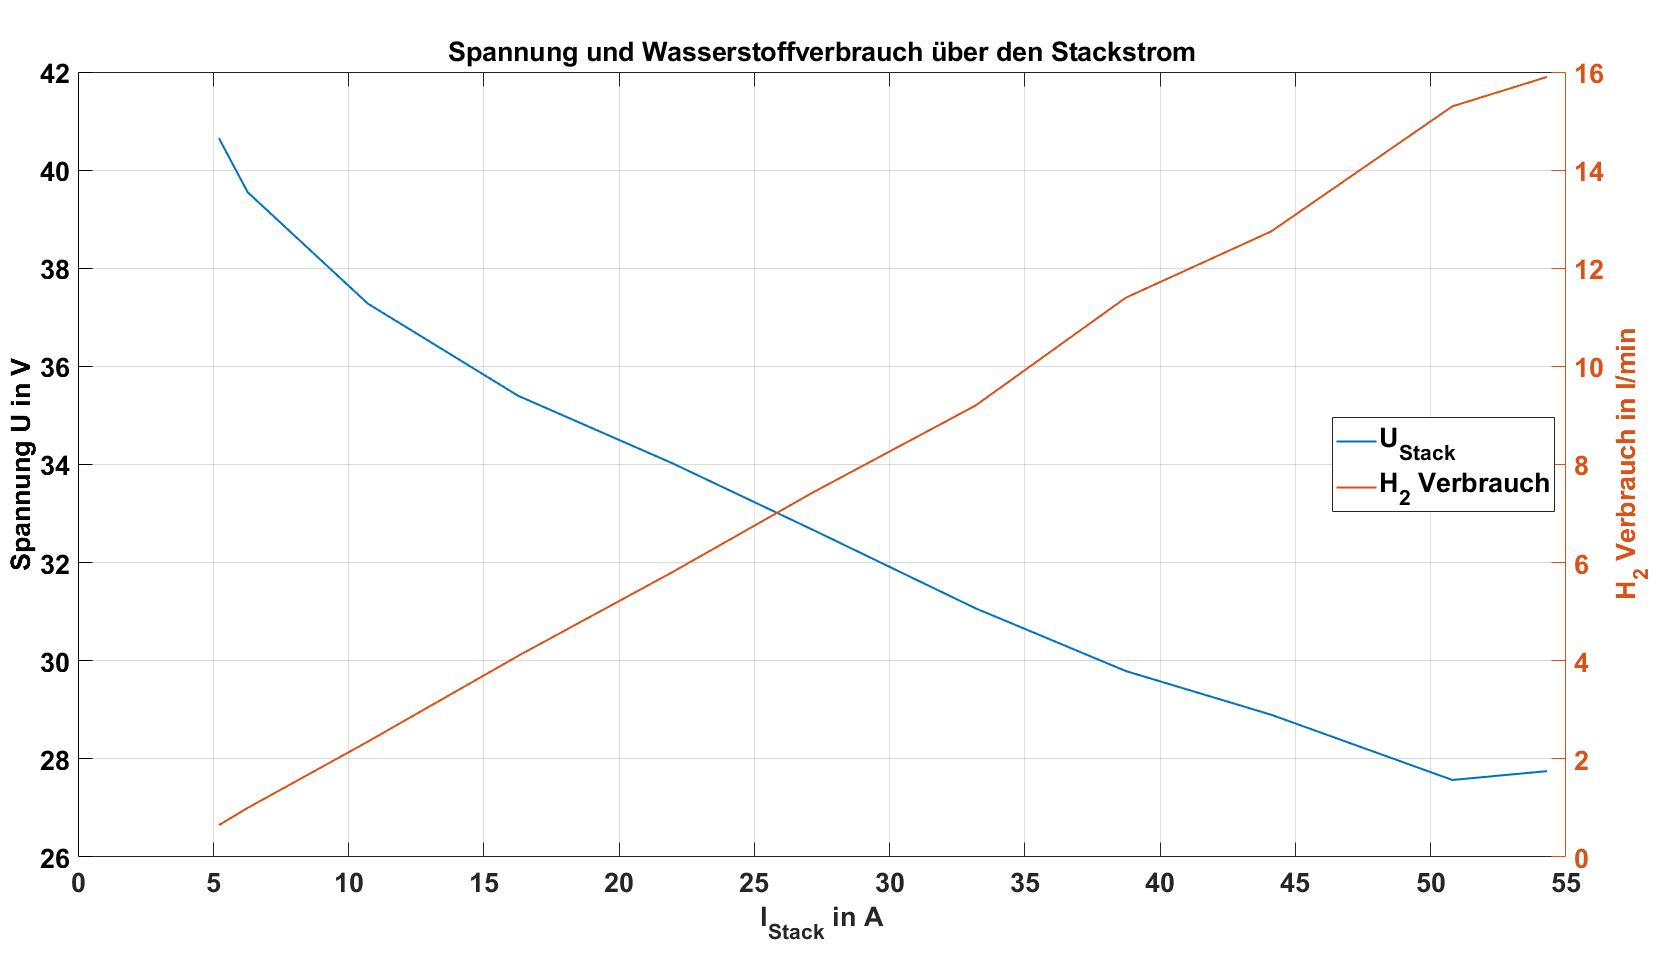
\includegraphics[width=0.8\textwidth]{Abbildungen/Aufgabe62_U und Vdot.png}
    \caption{Grafische Darstellung der Stackspannung und des Volumenstroms}
    \label{fig:230626_Stackspannung_Vdot}
\end{figure}

\begin{figure}[H]
  \centering
  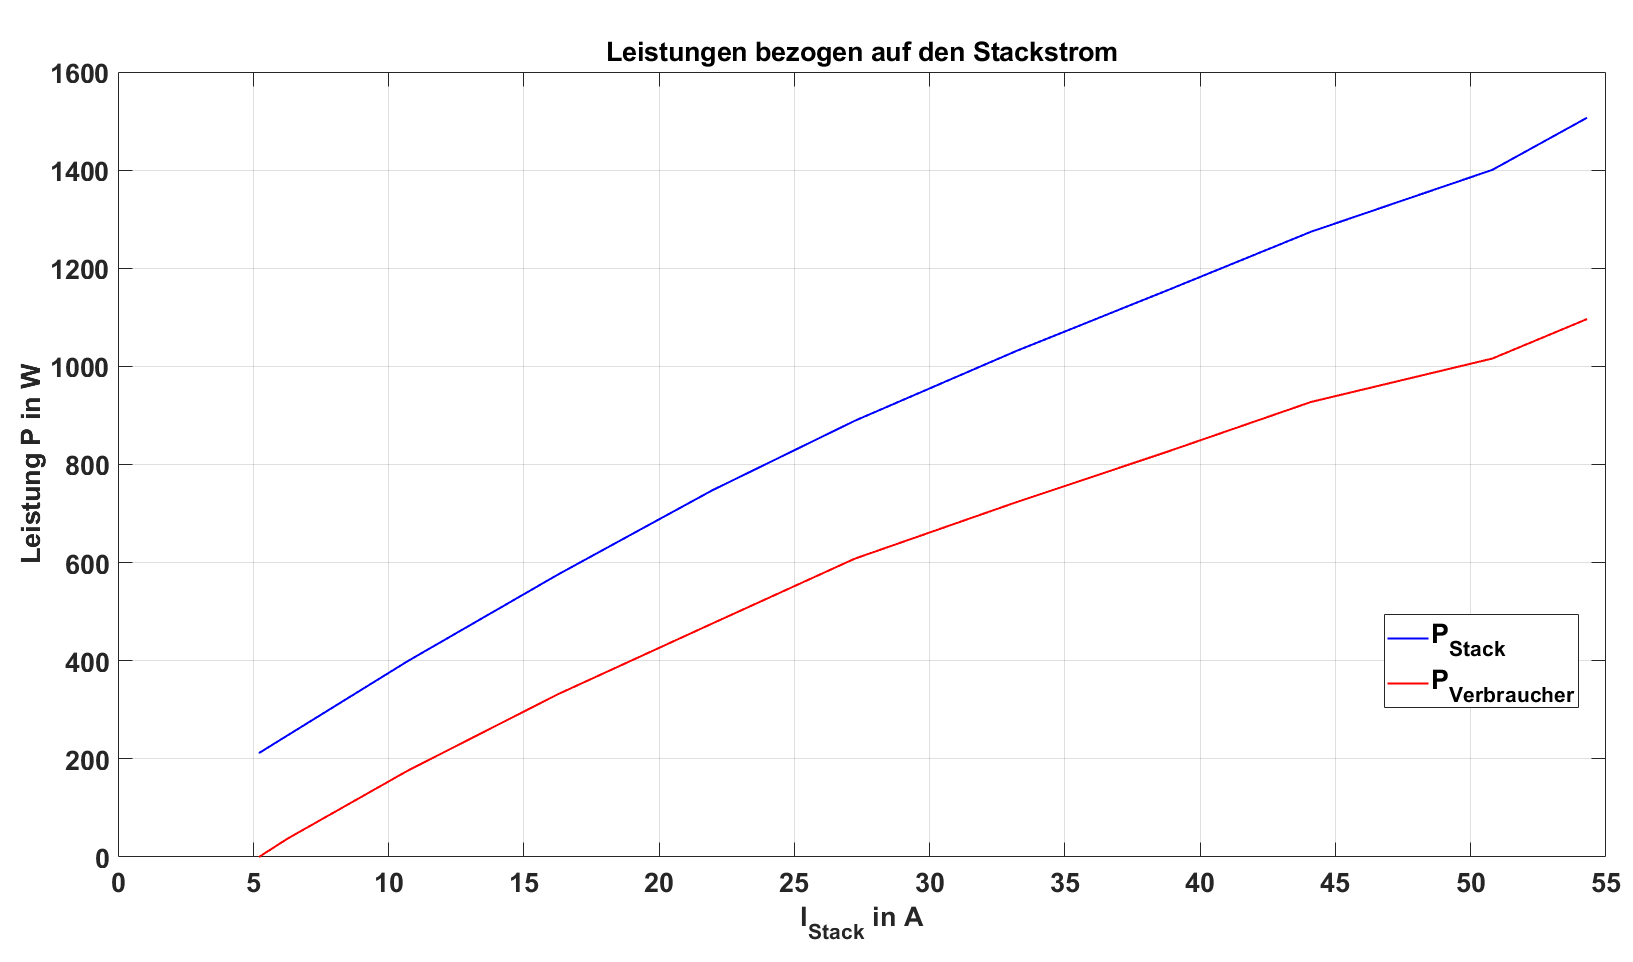
\includegraphics[width=0.8\textwidth]{Abbildungen/Aufgabe62_P.png}
  \caption{Grafische Darstellung der Stackleistung}
  \label{fig:230626_Stackleistung}
\end{figure}


\subsection{Grafische Darstellung einiger Messgrößen im Bezug zum Verbraucherstrom}

\begin{figure}[H]
    \centering
    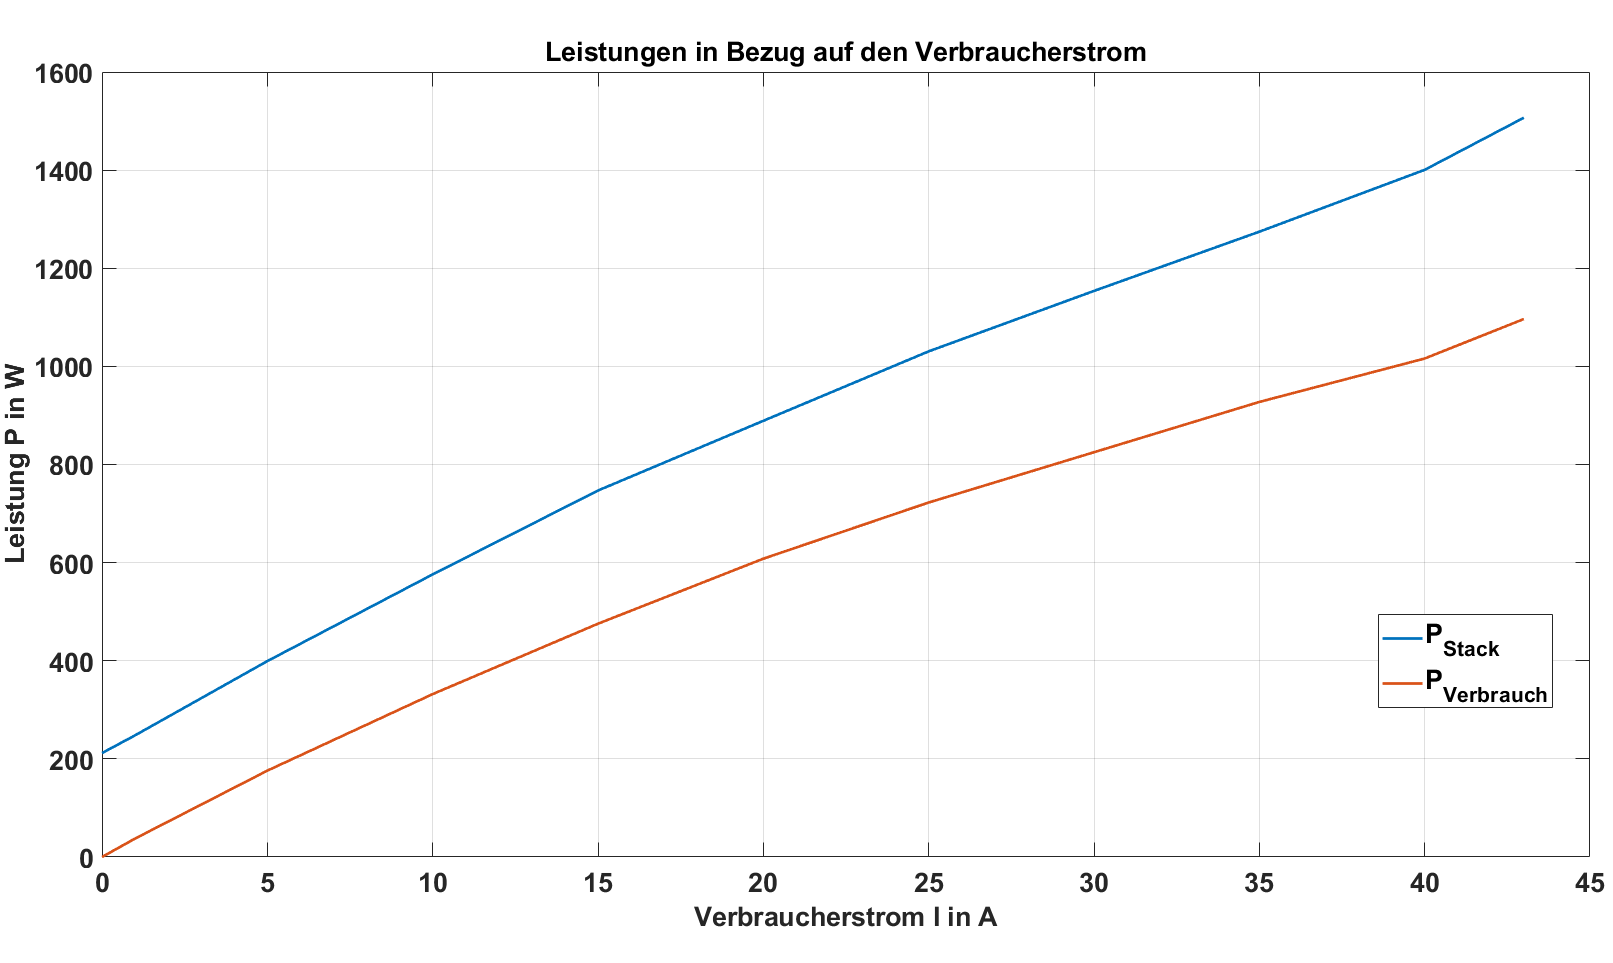
\includegraphics[width=0.8\textwidth]{Abbildungen/Aufgabe63_Leistungen_P.png}
    \caption{Grafische Darstellung der Leistungeneistung.}
    \label{fig:230626_Leistungen}
\end{figure}

\begin{figure}[H]
  \centering
  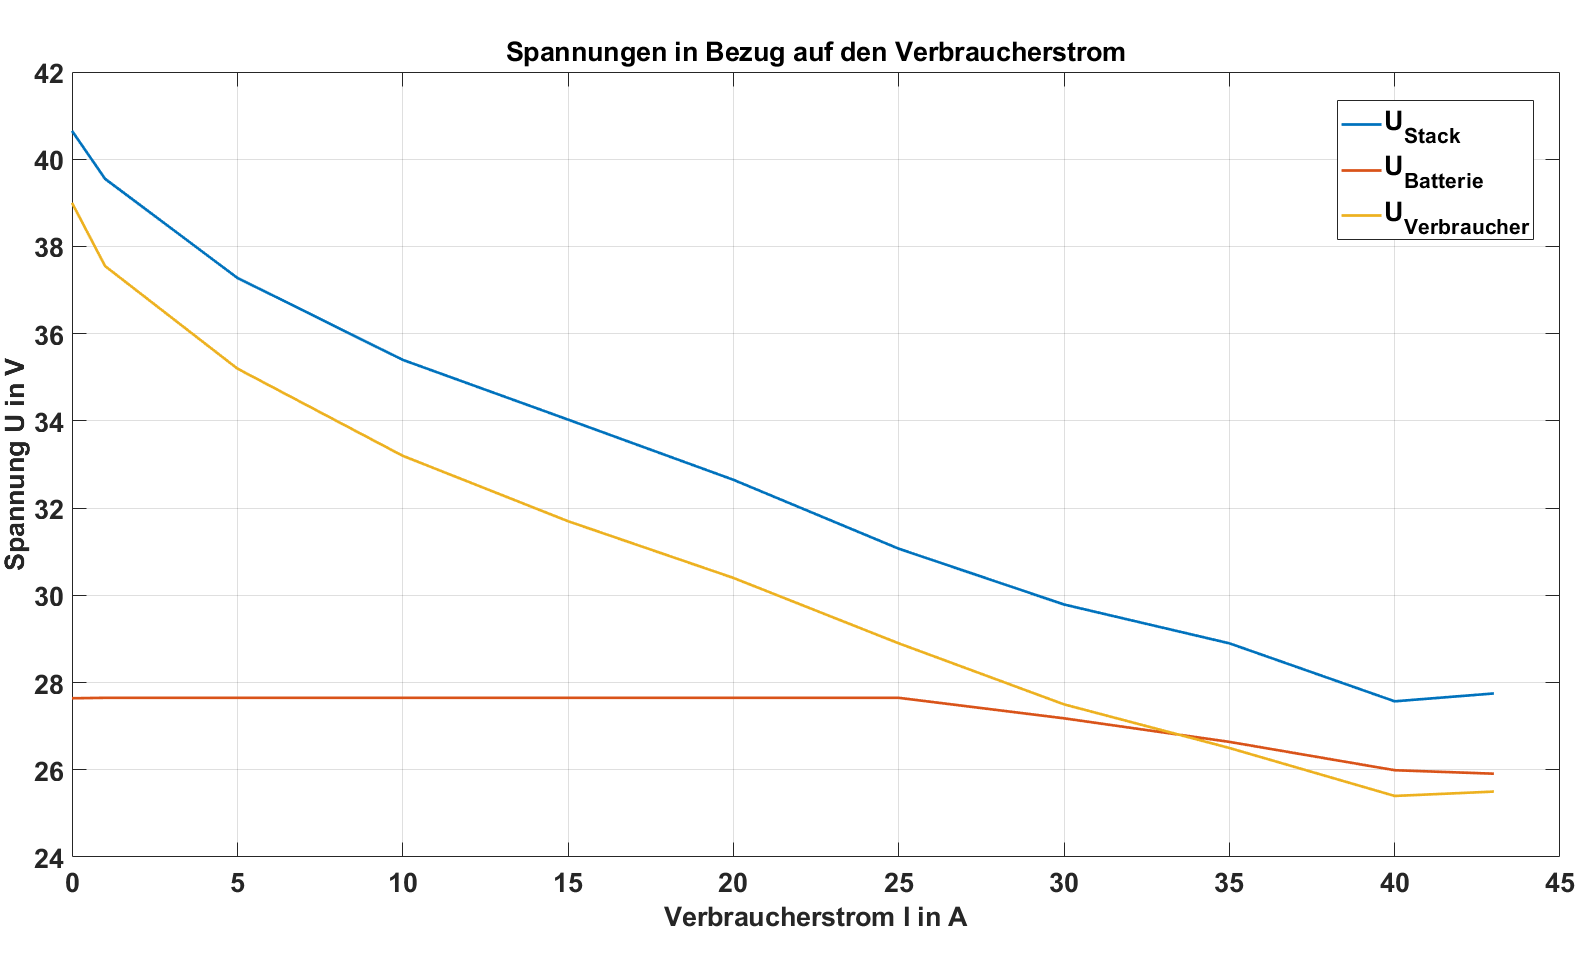
\includegraphics[width=0.8\textwidth]{Abbildungen/Aufgabe63_Leistungen_U.png}
  \caption{Grafische Darstellung der Stackspannung.}
  \label{fig:230626_Spannungen}
\end{figure}

\begin{figure}[H]
  \centering
  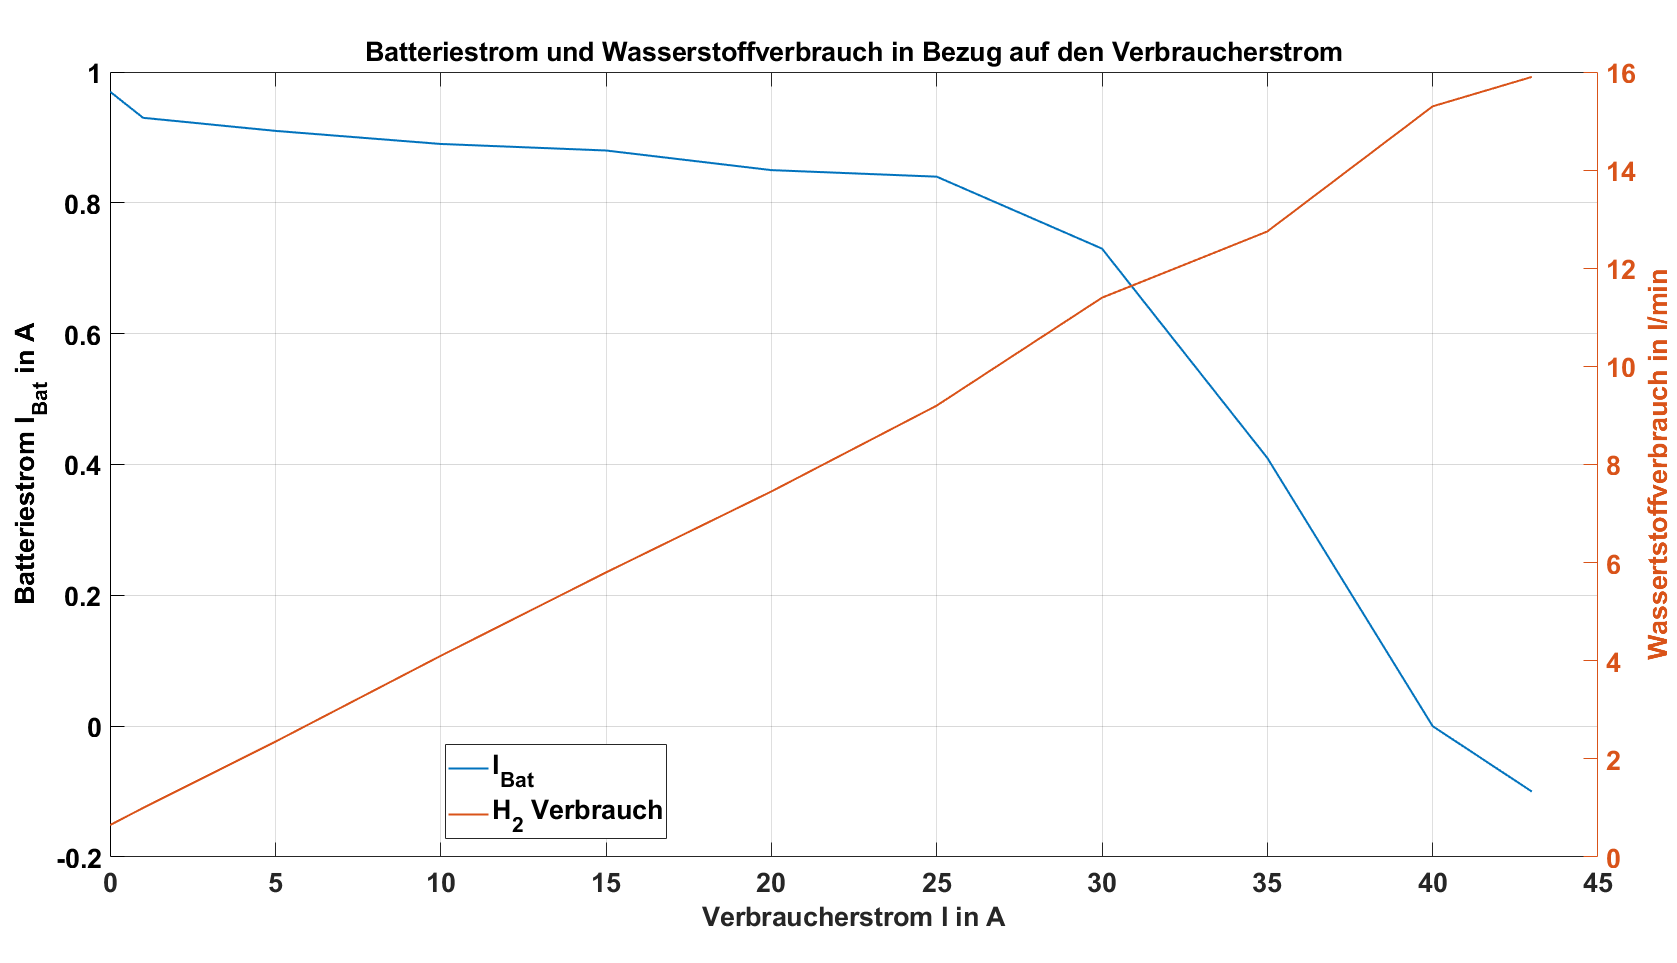
\includegraphics[width=0.8\textwidth]{Abbildungen/Aufgabe63_Leistungen_Ibat Vdot.png}
  \caption{Grafische Darstellung der Verbraucherleistung und des Wasserstoffverbrauchs.}
  \label{fig:230626_Ibat_Vdot}
\end{figure}

Um nun im nächsten Schritt den Wirkungsgrad des Stacks anhand des Heiz- und Brennwertes zu bestimmen, 
muss man den Wasserstoffverbrauch mit Hilfe des Heizwertes von $3 \frac{kWh}{m^3}$ und des Brennwerts von $3,54 \frac{kWh}{m^3}$ in eine Leistung umrechnen. 
Die tatsächlichen Leistungen an Stack und Gesamtsystem werden nun durch die vorher berechnete Leistung geteilt. 
Die folgende Gleichung zeigt diese Beispielhaft für den Stackwirkungsgrad:

\begin{equation}
 \eta= \frac{P_{Stack}}{H2_{Verbrauch_Stack}\cdot H2_{Brennwert}}
  \label{eq:230627_Beispiel_wirkungsgrad_Berechnung}
\end{equation}

$$\eta= \frac{1,506 kWh}{3,54 \frac{kWh}{m^3 }\cdot 0,954 \frac{m^3}{h}}=0,45$$

\begin{figure}[H]
    \centering
    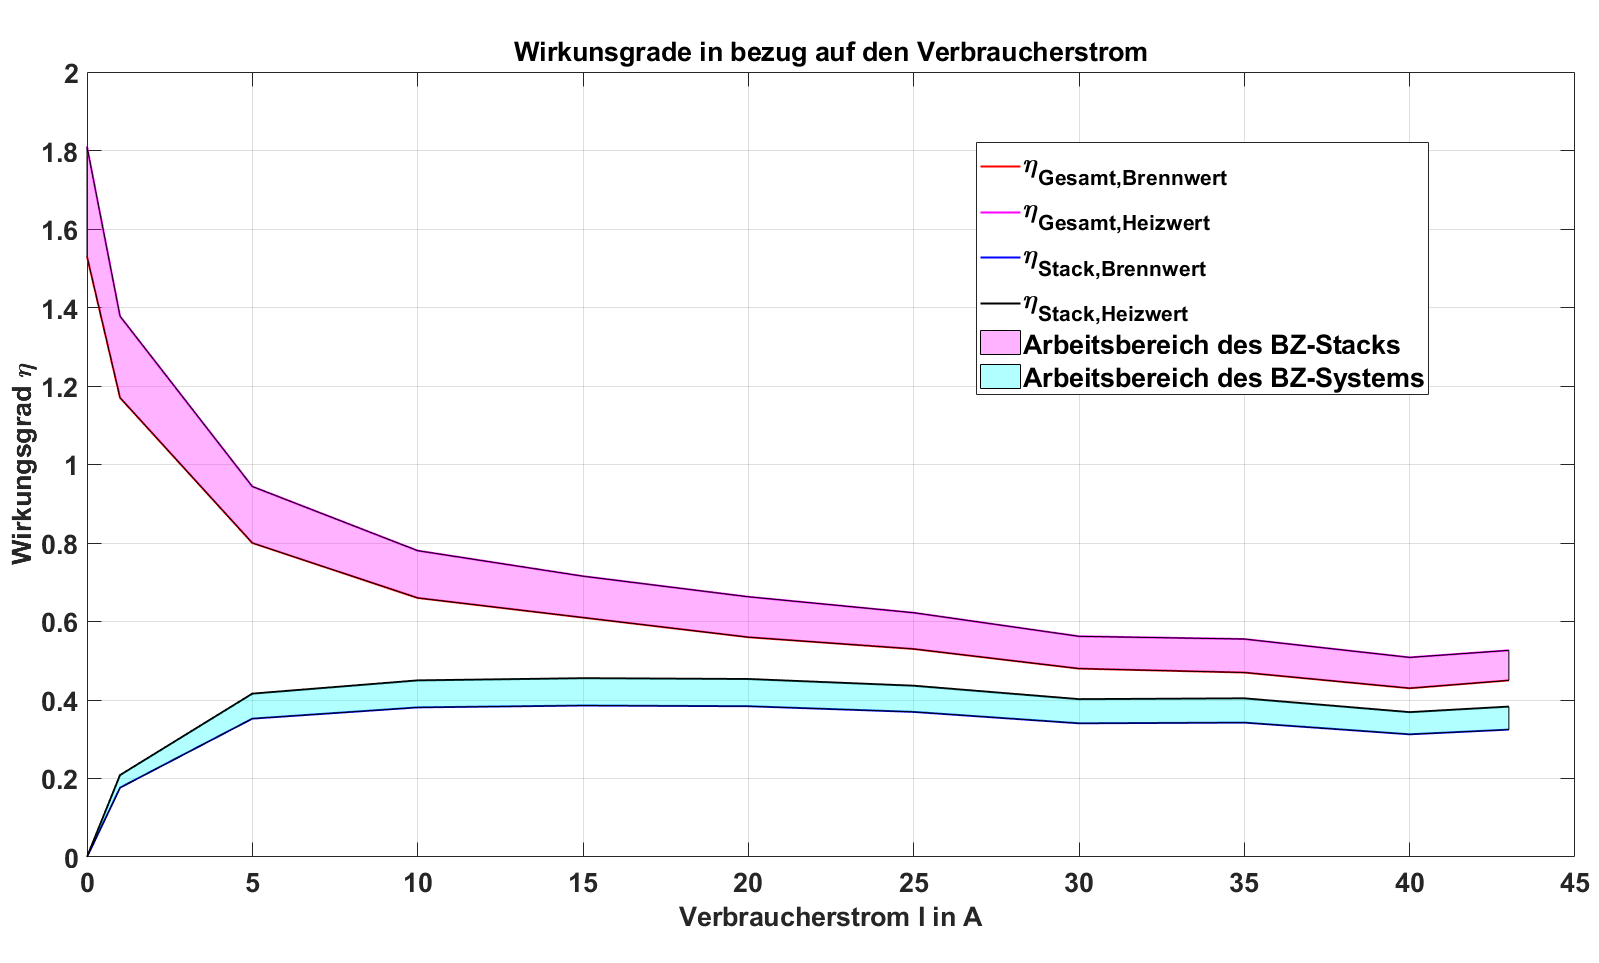
\includegraphics[width=0.8\textwidth]{Abbildungen/Aufgabe63_Wirkungsgrade.png}
    \caption{Wirkungsgradverlauf für den Stack und das gesamte System.}
    \label{fig:230626_Wirkungsgrade}
\end{figure}

Dabei entstehen die Wirkungsgradbänder bei Brennstoffzellen aufgrund von Verlusten in den Reaktionskinetiken, 
ohmschen Verlusten, Massentransportverlusten und den Betriebsbedingungen. 
Diese Faktoren beeinflussen die Leistungsfähigkeit und den Wirkungsgrad des Systems.
Die Art der Brennstoffzelle und die verwendeten Materialien spielen eine Rolle bei der Ausprägung der Wirkungsgradbänder. 
Unterschiedliche Betriebsparameter können zu variierenden Wirkungsgradbändern führen. 
Es gibt verschiedene Arten von Brennstoffzellen mit jeweils spezifischen Charakteristika und Herausforderungen im Hinblick auf Wirkungsgradbänder.


\subsection{Diskussion der Kurven}

\autoref{fig:230626_Stackspannung_Vdot} und \autoref{fig:230626_Spannungen} zeigt die unterschiedlichen Systemspannungen in Abhängigkeit des Stackstroms und des Verbraucherstrom. 
Zu erkennen ist die charakteristische Brennstoffzellen Spannungskennlinie, die in \autoref{fig:230626_Spannungen} genauer beschrieben wird. 
Die Stack- als auch die Verbraucherleistung steigen in Abhängigkeit des zugeführten Wasserstoffes proportional an, was in \autoref{fig:230626_Stackleistung}, \ref{fig:230626_Leistungen} und \ref{fig:230626_Ibat_Vdot} veranschaulicht wurde. 
Außerdem ist zu erkennen, dass bei steigendem Strom, sowohl die Stack- als auch die Verbraucherspannung leicht, absinken. Die lässt sich auch an dem Abfallen des Wirkungsgrades ablesen. 
In \autoref{fig:230626_Wirkungsgrade} ist der Verlauf des Wirkungsgrads des Stacks (schwarz und blau) sowie des Gesamtwirkungsgrads (rot und magenta) dargestellt. 
Der Wirkungsgrad wurde jeweils unter Verwendung des oberen und unteren Heizwerts berechnet, und die Toleranzbänder sind farblich gekennzeichnet. 
Es ist zu beachten, dass der Wirkungsgrad des Stacks deutlich über 100 Prozent liegt, was eigentlich nicht möglich ist und im krassen Gegensatz zum Verlauf des Gesamtwirkungsgrads steht.
Der Grund dafür liegt darin, dass die Brennstoffzelle bei Inbetriebnahme die Membranen spült, um sie von Unreinheiten und Ablagerungen zu befreien. 
Dieses Spülen der Membranen erfolgt mit Wasserstoff, wodurch für einen bestimmten Zeitraum deutlich mehr Wasserstoff zur Verfügung steht. 
Dadurch beginnt die Zellreaktion, bevor eine Leistungsabnahme des Verbrauchers eintritt. Dies führt zu den beschriebenen Wirkungsgraden des Stacks, die während des Startvorgangs über 1 liegen.


\subsection{Zusammenwirken von Brennstoffzellenstack, Batteriepuffer und Verbraucher}
Beim Regeln des Laststroms auf um die 43A schaltet sich die Brennstoffzelle im ungünstigesten Fall ab.
Die bereitgestellte Leistung der Brennstoffzelle reicht nicht aus um die Last auszugleichen und die Batterie fängt an sich zu entladen.
Wenn die Batterie nicht, schnell genug die nötige Ausgleichsleistung liefert, kommt es zum Ausfall.
Durch das Herunterregeln von 43 auf 20A wird die Brennstoffzelle in den Teillastetrieb versetzt.
Die Batterie wird von der Brennstoffzelle geladen.






\subsection{Teillastverhalten}

Die Wirkungsgrade werden nach \autoref{eq:230627_Beispiel_wirkungsgrad_Berechnung} mit Hilfe der Nutzleistung, dem Wasserstoffverbrauch und dem Heiz- und Brennwert von Wasserstoff berechnet. 

\begin{table}[H]
    \caption{Teillastwirkungsgrade der Brennstoffzelle}
    \centering
        \begin{tabular}[pos]{|c|c|c|}
            \hline
            \rowcolor[HTML]{70AD47} 
            I=20A   & $\eta_{Gesamt,Brennwert}$               & $\eta_{Gesamt,Heizwert}$   \\\hline\hline
            1. Messung  & 38,4\%                            & 45,3\%                            \\ \hline
            2. Messung  & 39,5\%                            & 46,6\%                            \\\hline
        \end{tabular}
        \label{tab:20230628_Teillastwirkungsgrade}
\end{table}

Die Brennstoffzelle hat einen sehr guten Teillastwirkungsgrad. In der zweiten Teillast-Messung ist die Brennstoffzelle wärmer als zuvor und hat ihre optimale Betriebstemperatur erreicht. Die Bauteile der Schaltung (Kompressor und Kühlung) sind eingeschwungen. Es werden bessere Werte als in der ersten Messung bei 20A erreicht. Außerdem auffällig ist der hohe Batteriestrom, dieser ist so hoch, da die Batterie vorher (durch hohe Lastströme) entladen und nun wieder aufgeladen wird. 

\newpage
\subsection{Energiebilanz für den Teillastfall}

\begin{figure}[H]
  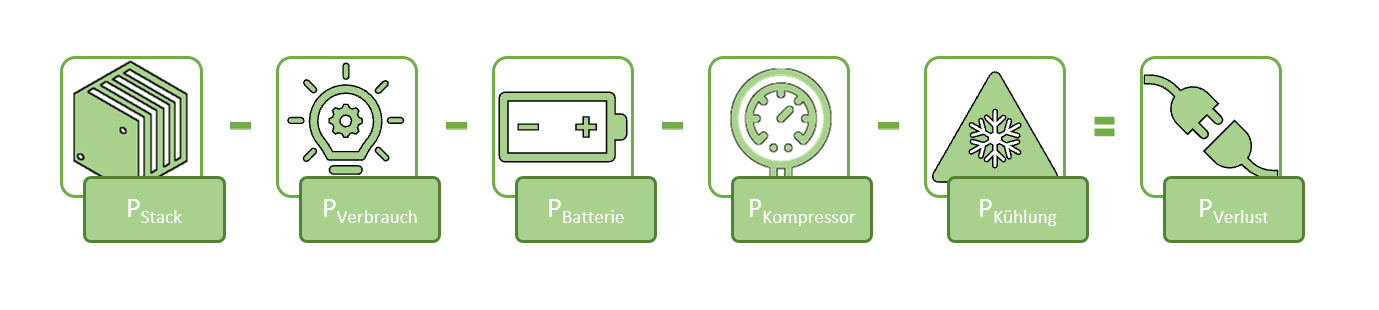
\includegraphics[width=1\textwidth]{BilanzFC.png}
\caption{Energiebilanz für Teillastfall}
\label{fig:20230630_Energiebilanz}
\end{figure}

In einem idealen System ist $P_{Stack}-P_{Gesamtverbrauch}=0$. Im betrachteten Teillastfall wird die Batterie wieder geladen, wodurch ein hoher Batterieladestrom entsteht und Energie entnommen wird.
Nach \autoref{fig:230618_U-I-Kennlinie} ist ebenfalls zu erkennen, dass sich die Batterie im Ladevorgang befindet. 
Im reellen System kommt es zu ohmschen und thermischen Verlusten. In der weiteren Betrachtung der Verluste werden diese als $P_{Verlust}$ vereinfacht zusammengefasst.
Durch Aufstellen der Energiebilanz können die Verluste im Teillastfall ermittelt werden.
In Abbildung \autoref{fig:20230630_Energiebilanz} ist Energiebilanz schematisch dargestellt.
\autoref{eq:20230630_Energiebilanz} gibt die Beziehung zwischen den einzelnen Systemkomponenten wieder.
\begin{equation}
  P_{Verlust} = P_{Stack}-P_{Verbrauch}-P_{Batterie}-P_{Kompressor}-P_{Kühlung}
\label{eq:20230630_Energiebilanz}
\end{equation}

Zur Ermittlung der Leistung werden die Messdaten aus \autoref{tab:20230616} genutzt.(Siehe Anhang)
Die Kompressor Leistung arbeitet bei 69\% und die Kühlung bei 40% der Volllast.
Die umgerechneten Leistungen werden in \autoref{tab:20230630_PTeillast} aufgeführt. 


\begin{table}[H]
  \centering
  \caption{Leistungen der Komponenten im Teillastversuch}
  \label{tab:20230630_PTeillast}
  \resizebox{\columnwidth}{!}{%
  \begin{tabular}{|l|l|l|l|l|l|}
  \hline
  \rowcolor[HTML]{70AD47} 
  \textbf{$P_{Stack}$} & \textbf{$P_{Verbrauch}$} & \textbf{$P_{Batterie}$} & \textbf{$P_{Kompressor}$} & \textbf{$P_{Kühlung}$} & \textbf{$P_{Verlust}$} \\ \hline
  \rowcolor[HTML]{E2EFDA} 
  965,545W              & 642W                      & 138W                     & 20W                        & 41,43W                  & 124,115W                \\ \hline
  \end{tabular}%
  }
  \end{table}

Mit den eingesetzten Werten aus \autoref{tab:20230630_PTeillast} werden die Leistungsverluste berechnet:
$$P_{Verlust}=965,545W-642W-138W-20W-41,43W=124,115W \approx 124W$$

$P_{Verlust}$ beträgt $\approx124W$.
